%%%%%%%%%%%%%%%%%%% vorlage.tex %%%%%%%%%%%%%%%%%%%%%%%%%%%%%
%
% LaTeX-Vorlage zur Erstellung von Projekt-Dokumentationen
% im Fachbereich Informatik der Hochschule Trier
%
% Basis: Vorlage svmono des Springer Verlags
%
%%%%%%%%%%%%%%%%%%%%%%%%%%%%%%%%%%%%%%%%%%%%%%%%%%%%%%%%%%%%%

\documentclass[envcountsame,envcountchap, deutsch]{i-studis}

\usepackage{makeidx}         	% Index
\usepackage{multicol}        	% Zweispaltiger Index
%\usepackage[bottom]{footmisc}	% Erzeugung von Fu�noten
\usepackage{float}
\restylefloat{table}

%%-----------------------------------------------------
%\newif\ifpdf
%\ifx\pdfoutput\undefined
%\pdffalse
%\else
%\pdfoutput=1
%\pdftrue
%\fi
%%--------------------------------------------------------
%\ifpdf
\usepackage[pdftex]{graphicx}
\usepackage{epstopdf}
\usepackage[pdftex,plainpages=false]{hyperref}
%\else
%\usepackage{graphicx}
%\usepackage[plainpages=false]{hyperref}
%\fi

%%-----------------------------------------------------
\usepackage{color}				% Farbverwaltung
%\usepackage{ngerman} 			% Neue deutsche Rechtsschreibung
\usepackage[english, ngerman]{babel}
\usepackage[latin1]{inputenc} 	% Erm�glicht Umlaute-Darstellung
%\usepackage[utf8]{inputenc}  	% Erm�glicht Umlaute-Darstellung unter Linux (je nach verwendetem Format)

%-----------------------------------------------------
\usepackage{listings} 			% Code-Darstellung
\lstset
{
	basicstyle=\scriptsize, 	% print whole listing small
	keywordstyle=\color{blue}\bfseries,
								% underlined bold black keywords
	identifierstyle=, 			% nothing happens
	commentstyle=\color{red}, 	% white comments
	stringstyle=\ttfamily, 		% typewriter type for strings
	showstringspaces=false, 	% no special string spaces
	framexleftmargin=7mm, 
	tabsize=3,
	showtabs=false,
	frame=single, 
	rulesepcolor=\color{blue},
	numbers=left,
	linewidth=146mm,
	xleftmargin=8mm
}
\usepackage{textcomp} 			% Celsius-Darstellung
\usepackage{amssymb,amsfonts,amstext,amsmath}	% Mathematische Symbole
\usepackage[german, ruled, vlined]{algorithm2e}
\usepackage[a4paper]{geometry} % Andere Formatierung
\usepackage{bibgerm}
\usepackage{array}
\hyphenation{Ele-men-tar-ob-jek-te  ab-ge-tas-tet Aus-wer-tung House-holder-Matrix Le-ast-Squa-res-Al-go-ri-th-men} 		% Weitere Silbentrennung bei Bedarf angeben
\setlength{\textheight}{1.1\textheight}
\pagestyle{myheadings} 			% Erzeugt selbstdefinierte Kopfzeile
\makeindex 						% Index-Erstellung


%--------------------------------------------------------------------------
\begin{document}
%------------------------- Titelblatt -------------------------------------
\title{Digitalisierung und Bildung: Risiken digitaler Informationstechnik}
\project{Ausarbeitung zur Vorlesung Wissenschaftliches Arbeiten}
%--------------------------------------------------------------------------
\supervisor{Prof. Vorname Name} 		% Betreuer der Arbeit
\author{Bearbeiter 1: Marc Meyer \\Bearbeiter 2: Lionel Schroeder \\Bearbeiter 3: Tom Walter}							% Autor der Arbeit
\groupid{67}
\address{Schneidershof 1, 54293 Trier} 							% Im Zusammenhang mit dem Datum wird hinter dem Ort ein Komma angegeben
\submitdate{29.5.18} 				% Abgabedatum
%\begingroup
%  \renewcommand{\thepage}{title}
%  \mytitlepage
%  \newpage
%\endgroup
\begingroup
  \renewcommand{\thepage}{Titel}
  \mytitlepage
  \newpage
\endgroup
%--------------------------------------------------------------------------
\frontmatter 
%--------------------------------------------------------------------------
\kurzfassung

%% deutsch
\paragraph*{}
Traditionelle Bildung versagt. Die neuen Technologien k�ndigen eine neue �ra der Bildung an. Unsere Arbeit verweist auf die H�rden der Implementierung digitaler Hilfsmittel in Lehrveranstaltungen. Anfangs behandeln wir die Implementierung von Belohnungssystemen im Lernprozess, mit dem Resultat, dass Sch�ler motivierter sind, jedoch keine positive Korrelation zwischen Technologie und Leistung existiert. Zudem vergleichen wir die Leistung und Schreibmotorik der altmodischen Sch�ler zu der von Technologie gesegneten Generation Z. Trotz elektronischer Hilfsmittel verschlechtert sich die Grammatik. Abschlie�end zeigen wir, dass diese Technologien die Ursache f�r erh�hte Depressionserscheinungen sowie Konzentrationsmangel bei Jugendlichen sind und deswegen f�r eine schw�chere akademische Leistung sorgen.

 			% Kurzfassung Deutsch/English
\tableofcontents 						% Inhaltsverzeichnis
%--------------------------------------------------------------------------
\mainmatter                        		% Hauptteil (ab hier arab. Seitenzahlen)
%--------------------------------------------------------------------------
% Die Kapitel werden in separaten .tex-Dateien abgelegt und hier eingebunden.
\chapter{Einleitung und Problemstellung}

Motivations\- und Anteilnahme M�ngel sind vorrangige Probleme im aktuellen Schulwesen und k�nnten durch Technologie gel�st werden. Einerseits gibt es vielversprechende Initiativen, beispielsweise bildungsorientierte Spiele zu entwerfen, um den Spa� am Lernen zu wecken. 
Andererseits erweist sich die effektive Integration spielerischer Komponenten als kostenspielig und aufwendig. 
Au�erdem ist der positive Impakt vom Einsatz neuer Technologien im Schulwesen umstritten. 
Der Bereich der Textverarbeitungsprogramme ist beispielsweise problematisch, denn meistens haben diese Programme eine W�rterkorrektur implementiert, auf die sich manche Menschen zu sehr verlassen und eventuell die F�higkeit verlieren, sich selbst �ber die Korrektheit der Eingabe zu vergewissern. 
Durch regelm��iges Verwenden dieser Software verlernen Nutzer ebenfalls die Handschrift.
 \"Der Mensch ist, was er als Mensch sein soll, erst durch Bildung\" -Wilhelm Friedrich. 
 Die Revolution des Bildungswesen ist ein stets relevantes Thema in der Politik und Gesellschaft. 
 Die gegenw�rtige Initiative in der Politik besteht darin, der Jugend das Lernen durch Einsatz neuer Software und Hardware zu erleichtern. 
 E-Learning ist gem�� Studien eine verhei�ungsvolle Antwort auf Streitpunkte kontempor�rer Bildungsmechanismen. 
 Nichtsdestotrotz bringt die Digitalisierung sowohl Risiken als auch Erfolge mit sich. Ein weiteres wichtiges Thema sind die psychologischen Abdr�cke der Technologien. Eine Digitalisierung der Bildung f�hrt automatisch zu einem vermehrten Nutzen von Computern, Smartphones und anderen technischen Hilfsmittel wie Tablets. Der Zustand der Psyche eines Studenten wirkt sich direkt auf seine akademische Leistung aus. Es ist notwendig sich mit den Auswirkungen jener Hilfsmittel mit den Studenten auseinanderzusetzen. 
\chapter{Futuristisches Lernen}
\section{Spielerisches Lernen}
Die Kanzlerin Angela Merkel lie� sich auf der Gamescom Minecraft, das Flagship-Produkt unter den Lernspielen, zeigen. Das aus Bl�cken bestehende Spiel hilft Kindern weltweit die Grundz�ge der Physik und der Architektur spielerisch zu erlernen. Es wird zum Beispiel in schwedischen Grundschulen als Fach angeboten
\cite{julius}. 
Der Nutzen des spielerischen Lernens gewinnt kontinuierlich an Bedeutung. Wenn das Lernen f�r Sch�ler interessant gestaltet wird, ist der Lernerfolg noch besser
\cite{[2]}.
Da traditioneller Unterricht von vielen Studenten und Sch�lern als langweilig und ineffizient empfunden wird, liegt der innovative Fokus in der Bildung auf dem Entgegenkommen von Motivations- und Anteilnahme M�ngel im Schulwesen.
Beispiel daf�r ist die sogenannte "Kahoot"-App, die es erm�glicht Quizze zu erstellen und zu spielen. Lernende antworten auf ihren Tablets oder Smartphones mit einem Nicknamen. Besonders effektiv sind die Quizzes am Anfang oder am Ende des Unterrichts zur Wiederholung des letzten Stoffes oder um zu sehen ob der neue Stoff gut verstanden wurde. Die Sch�ler lernen durch spielerischen Wettbewerb, was auch der gr��te Vorteil der App ist. Sie m�gen das Layout, die Musik und die Spannung durch die limitierte Zeitvorgabe. Nach jeder Frage wird die Platzierung angezeigt die den Ehrgeiz der Teilnehmer verst�rkt, und dank der Nicknamen wird niemand blo�gestellt
\cite{[3]}.
Bildungsorientierte Spiele sind eine vielversprechende potentielle L�sung zu den Motivationsproblemen aufgrund ihrer F�higkeit, nicht nur Wissen anzueignen, sondern auch Probleml�sung, Kommunikation und Kollaboration zu f�rdern. Spiele haben eine au�ergew�hnliche Motivationskraft indem sie Gebrauch von Techniken machen, die den Nutzer zur Interaktion durch blo�e Freude am Spiel oder um zu gewinnen, motivieren.
Um das Potential der Gamifikation zu verstehen, m�ssen wir uns Gedanken dar�ber machen, wie Belohnungssysteme aus Spielen das Verhalten des Nutzers in der Praxis beeinflussen. Spiele bieten komplexe Systeme mit festen Regeln welche Spieler durch aktive Experimentation und Entdeckung zum Erforschen bewegen. Einfacher gesagt: Spiele leiten Spieler durch den Prozess der Meisterschaft der Aufgabestellung und halten sie mit potentiell schwierigen Aufgaben besch�ftigt, die sich mit der Zeit an die Kapazit�t des Spielers anpassen.
Die Tabelle [4] dokumentiert die am h�ufigsten dokumentierten Gamifikation-Design Prinzipien.
\begin{table}
\begin{tabular}{|p{5cm}|p{5cm}|p{5cm}|}
\hline
Design Prinzipien & Spielmechaniken & Wissenschaftliche Artikel \\
\hline
Rapides Feedback (sofortige und klare, anstatt langzeitige und wage, "Belohnungen", Ergebnisse)& &  (Lee und Hammer, 2011) (Nah, et al., 2014) (Zichermann und Cunningham, 2011) (Kapp, 2012) (Simoes, D�az und Fernandez, 2013)\\
\hline
Erkennbarer Status (Ruf, soziale Kredibilit�t und Anerkennung & Punkte, Abzeichen, Bestenlisten, Avatare &  (Lee und Hammer, 2011) (Deterding, 2013) (Simoes, D�az und Fernandez, 2013)\\
\hline
Entscheidungsfreiheit &  & (Lee und Hammer, 2011) (Iosup und Epema, 2014) (Deterding, 2013) (Simoes, Diaz und Fernandez, 2013)\\
\hline
Freiheit fehlzuschlagen (viele Versuche, wenig Risiko) &  & (Lee und Hammer, 2011) (Kapp, 2012) (Deterding, 2013) (Gordon, Brayshaw und Grey, 2013)\\
\hline
Soziales Engagement & Abzeichen, Levels, Statistiken & \\
\hline
\end{tabular}
\end{table}

Lernende reagieren in Spielen sehr positiv auf Rapides Feedback. In Spielen erh�lt man sofort eine Belohnung oder einen Bericht wenn man zum Beispiel eine Mission erf�llt oder gegen einen Gegner gewinnt oder verliert. Dadurch werden die Spieler motiviert am Ball zu bleiben und es noch besser zu machen.Erkennbarer Status ist in heutigen Spielen nicht mehr wegzudenken. Es geh�rt allgemein auch zu den wichtigsten menschlichen Motivationstrieben. Durch Punkte, Abzeichen oder Bestenlisten l�sst sich sichtbarer Status einfach in Spielen als auch in der Bildung implementieren. Drei weitere wichtige Spielprinzipien sind Entscheidungsfreiheit, soziales Engagement und die Freiheit, fehlschlagen zu d�rfen. Lernende als auch Spieler reagieren positiv auf ein Umfeld, in welchem sie miteinander kommunizieren und Kreativit�t durch Flexibilit�t aus�ben k�nnen. Die Freiheit, fehlzuschlagen und ohne gro�es Risiko zu arbeiten, ist im Zusammenhang mit Bildung sehr umstritten, jedoch reagieren Jugendliche positiv auf ein solches Umfeld und es kann ihre Motivation sogar steigern.
\section{Performanz in Rechnerr�umen}
Ein solches Spiel zu entwerfen, welches den Nutzern alle relevanten Inhalte beibringt und Spa� macht, erweist sich allerdings als sehr aufwendig und kostenspielig? \cite{[5]}.
Eine Anwendung im Klassenraum setzt entsprechende technische Infrastruktur und qualifizierte Fachkraft voraus.
W�hrend die Idee der Gamifikation eine sehr optimistische Auswirkung auf das Schulwesen, was Produktivit�t und Motivation angeht, projiziert, ist der positive Impakt von Technologie, insbesondere von Rechnern und Internet im Klassensaal oder Zuhause fragw�rdig. Der Fokus sollte darauf liegen, den anspruchsvollen Umgang mit der Technologie in einer Art und Weise zu f�rdern, die das Aneignen von Unterrichtsmaterial vereinfacht.
 
Im Durchschnitt ist die Performanz schlechter umso mehr mit Rechnern ger�stete Klassenr�ume von Studenten genutzt werden. Das stimmt nicht f�r jedes Land. Ausnahmen sind Australien und D�nemark , in welchen kaum ein Unterschied zwischen Sch�lern, die diese nutzen und denen, die sie nicht nutzen, liegt. Allerdings gibt es kein Land in welchem der Nutzen von Computern mit besserer Performanz assoziiert wird. Das k�nnnen wir anhand des folgenden Figur 3.1 zeigen, welcher die Digitale Leseperformanz in Relation zum Rechnergebrauch in Kursen in der Unterrichtssprache darstellt.\cite{[6]}
Auf dem Graphen erkennen wir, dass im Durchschnitt der Rechnergebrauch in Kursen in der Unterrichtssprache mit einer schlechteren Digitalen Leseleistung korreliert. Erstaunlicherweise gibt es jedoch Ausnahmen, demnach gibt es keine derartige Korrelation in Australien und D�nemark. Auch wenn die Leistung durch die Rechner keine positive Auswirkung in den beiden L�ndern bewirkt, beweist es aber dass es nicht nur einseitig schlecht, sondern ausbauf�hig ist.\cite{[7]}
\begin{figure}
\centering
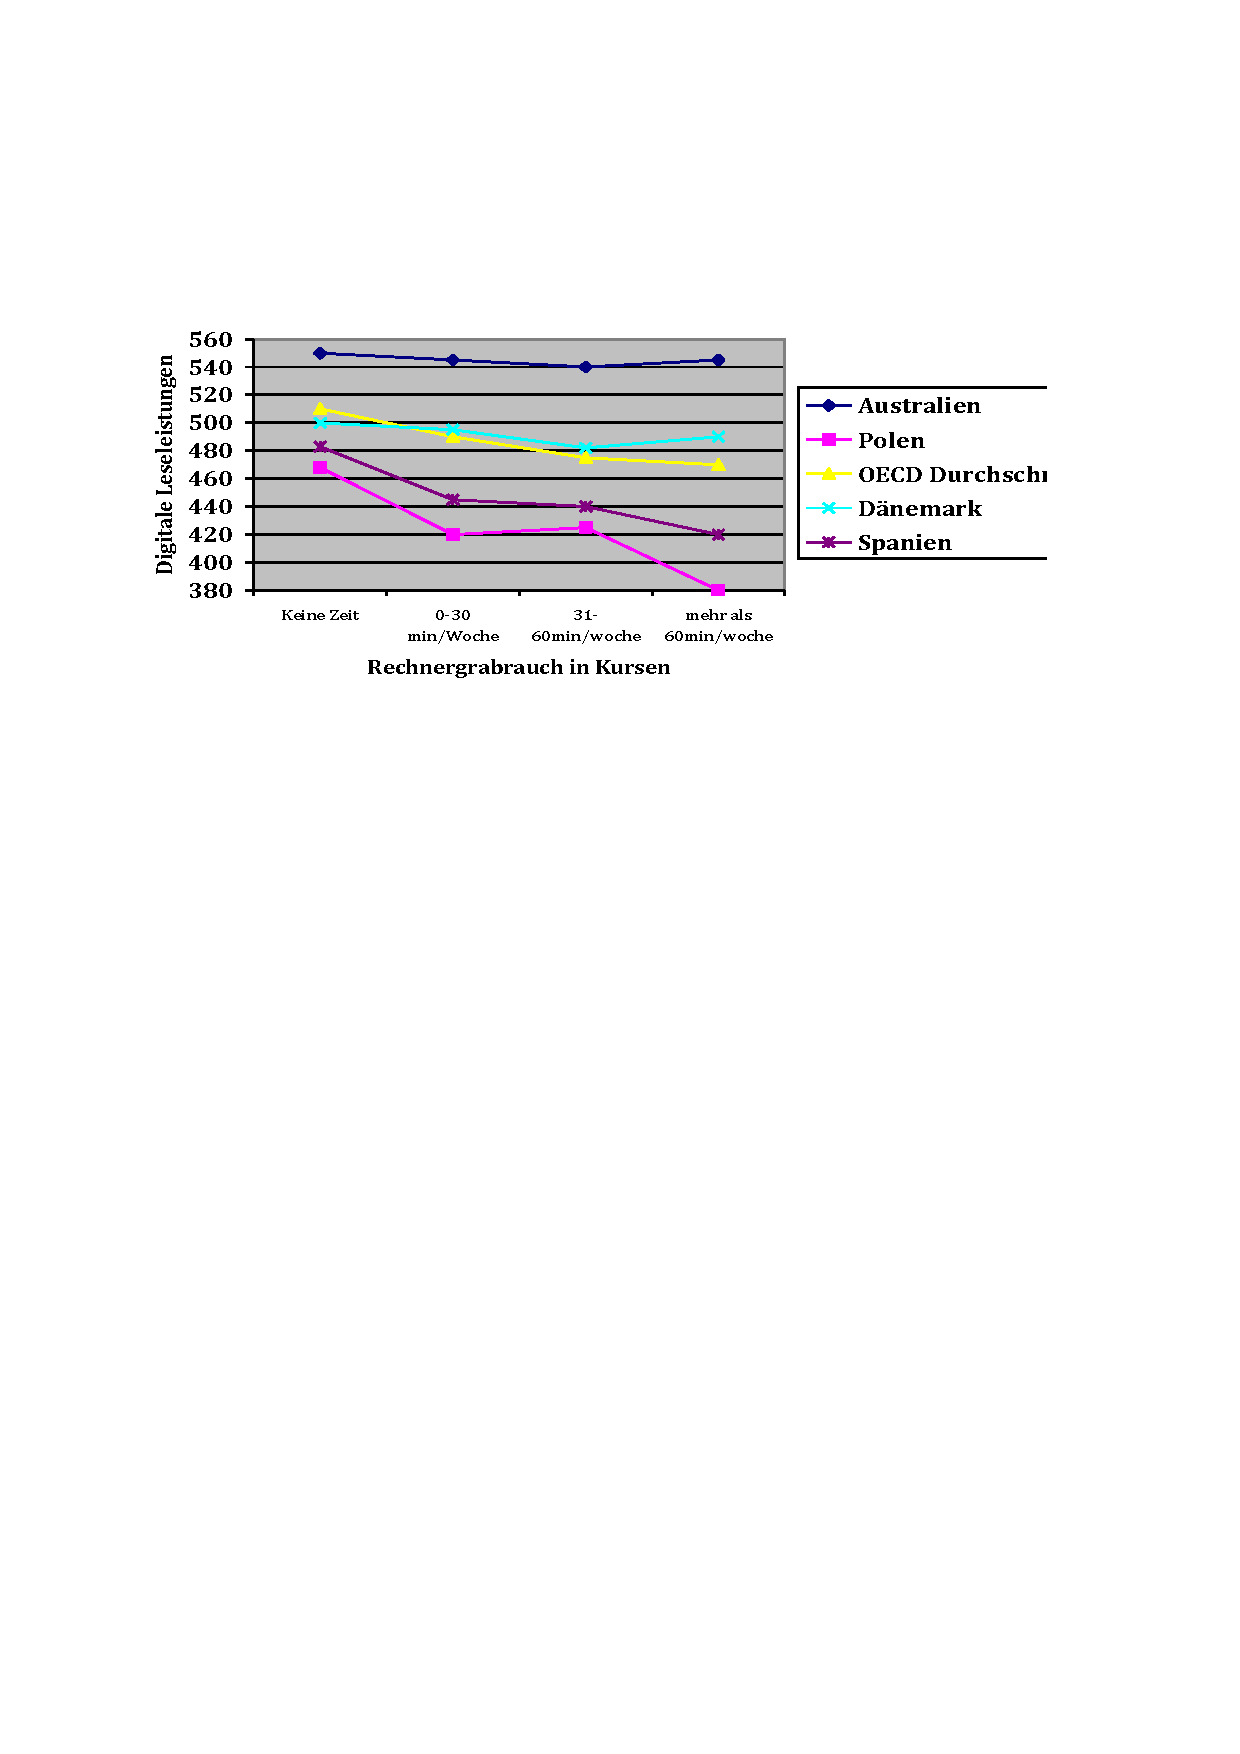
\includegraphics[scale=1]{images/Mappe1.pdf}
\end{figure}
Im Durchschnitt ist die Performanz schlechter umso mehr mit Rechnern ger�stete Klassenr�ume von Studenten genutzt werden. Das stimmt nicht f�r jedes Land. Ausnahmen sind Australien und D�nemark, in welchen kaum ein Unterschied zwischen Sch�lern, die diese nutzen und denen, die sie nicht nutzen, liegt. Allerdings gibt es kein Land in welchem der Nutzen von Computern mit besserer Performanz assoziiert wird. Das k�nnnen wir anhand des folgenden Graphen zeigen, welcher die Digitale Leseperformanz in Relation zum Rechnergebrauch in Kursen in der Unterrichtssprache darstellt
Die Tatsache, dass nahezu alle Studenten Zugang zu Rechnern haben hei�t noch lange nicht dass sie diesen auch nutzen. Und wenn sie ihn nutzen, dann oft nur um im Internet zu browsen oder Emails zu lesen. Gem�� einer Studie \cite{[8]}.

ICILS 2013 �ber Computerskills ist der Prozentsatz von Studenten mit der niedrigsten Kompetenz bedeutend.Fast die H�lfte der Jugendlichen in Deutschland ordnet sich in der mittleren Komepenzstufe III ein (~45 Prozent). Diese Sch�ler sind im Stande, ?unter Anleitung Dokumente zu bearbeiten und simple Informationsprodukte zu erstellen.? Ungef�hr ein Dritte aller deutschen Sch�ler schaffen es in die zwei niedrigsten Komepenzstufen I und II. Sie besitzen also eine sehr niedrige Kompetenz in Bezug auf ihre Fertigkeiten und Wissensbest�nde im Umgang mit Technologien und Informationen. Die oberste Kompetenzstufe f�llt mit einem Anteil von 1,5 Prozent sehr gering aus. \cite{[8]}.
\begin{table}
\begin{tabular}{|l|p{7cm}|}
\hline
Kompetenzstufe I & Unzureichende, vorwiegend rezeptive Fertigkeiten und sehr einfache Anwendungskompetenzen\\
\hline
\hline
Kompetenzstufe II & Grundlegende Wissensbest�nde und Fertigkeiten hinsichtlich der Identifikation von Informationen und der Bearbeitung von Dokumenten \\
\hline
\hline
Kompetenzstufe III & Angeleitetes Ermitteln von Informationen und Bearbeiten von Dokumenten sowie Erstellen einfacher Informationsprodukte \\
\hline
\hline
Kompetenzstufe IV & Eigenst�ndiges Ermitteln und Organisieren von Informationen und selbstst�ndiges Erzeugen von Dokumenten und Informationsprodukten \\
\hline
\hline
Kompetenzstufe V & Sicheres Bewerten und Organisieren selbstst�ndig ermittelter Informationen und Erzeugen von inhaltlich sowie formal anspruchsvollen Informationsprodukten\\
\hline


\end{tabular}
\end{table}
\chapter{Chapter2}


\section{Grammatik}

Im 21. Jahrhundert, ist das Schreiben und Lesen wichtiger als Sprechen und Zuh�ren. 
Ein Individuum, welches �ber keine guten Schreib- und Lesekenntnisse verf�gt kann in der Industrie 4.0 Probleme am Arbeitsmarkt haben. 
Angestellte arbeiten von Zuhause und die verschiedenen Kollegen m�ssen sich anhand elektronischer Telekommunikation Informationen mitteilen oder austauschen. 
Laut einer Studie \cite{Sassone} aus England von Global Lingo w�rden 59 Prozent der 1029 gefragten Briten keinen Service einer Firma nutzen die Rechtschreibfehler in ihrem Marketing Materialien vorweisen \cite{Hesse}. 

Der Online Entrepreneur Charles Duncombe behauptet, dass Rechtschreibfehler Kunden abschrecken und die Webseite als nicht glaubw�rdig erscheinen lassen w�rden .

Die Forsa Gesellschaft hat im Jahr 2014 in einer Umfrage \cite{forsa} verschiedenen Sprachwissenschaftlern aus Deutschland die Frage gestellt, 
ob die Digitalisierung die Deutsche Sprache beeinflussen w�rde. Von der Tabelle 3.1 sind 62 Prozent der gefragten Sprachwissenschaftler davon �berzeugt, 
dass die digitale Kommunikation die Deutsche Sprache beeinflusst. 33 Prozent gehen davon eher weniger aus, und 4 Prozent �berhaupt nicht.
22 Prozent der Sprachwissenschaftler mit der Ansicht, die Digitalisierung habe einen kleineren Einfluss auf die Sprache behaupten,
dass die Vermischung von gesprochener und geschriebenerSprache durch Abk�rzungen und Floskeln eine Entstehung von Neologismen provoziert. 
Es entsteht eine �nderung um 19 Prozent bei der Rechtschreibung, Grammatik und Interpunktion. 
17 Prozent behaupten, dass dadurch neue Formen der Kommunikation entstehen. 14 Prozent behaupten, dass eine Ver�nderung des Kommunikationsverhalten zu sehen ist, 
wie beispielsweise bei Emails und Textnachrichten.
\renewcommand{\arraystretch}{2}
\begin{table}[H] 
\small
\centering
\begin{tabular}{|l|p{1cm}|} 
\hline
Abkurzungen, Floskeln, neue Worter, kurzere S�tze                      & \centering{22} \cr \hline
Vermischung von Mundlichkeit und Schriftlichkeit                          & \centering{22} \cr \hline
Ver�nderung der Grammatik, Rechtschreibung, Interpunktion                 & \centering{19} \cr \hline
Ver�nderung der Kommunikationsbedingungen                                 & \centering{17} \cr \hline
Ver�nderung des Kommunikationsverhaltens, mehr schriftliche Kommunikation & \centering{14} \cr \hline
\end{tabular}

\caption{Ver�nderung der deutschen Sprache durch die Digitlisierung}
\label{my-label}
\end{table}


Die Nutzung digitaler Ger�te wie Smartphones oder Tablettes tragen zum Verlernen der Grammatik und Rechtschreibung bei. 
Sch�ler schreiben mit ihren Peers in verk�rzten Texten und Abk�rzungen wie 'OMG' was f�r Oh mein Gott steht.


Drew Cingel und S. Shyam Sundar von der Universit�t aus Pennsylvania meinen dazu, 
dass die jeweiligen Sch�ler vielleicht nicht mehr den Unterschied zwischen dem Schreiben mit der grammatikalisch korrekten Regelung und Umgangssprache differenzieren k�nnen. 
Cingel und Sundar haben dies empirisch belegt, indem sie Sch�ler der Mittelstufe einen Grammatik Test haben schreiben lassen. Zus�tzlich haben sie eine Umfrage konzipiert, 
die zeigen sollte, das Textnachrichten Angewohnheit der Sch�ler sind. Das Resultat der Umfrage war, wie bef�rchtet, 
dass man mit Hilfe der Textnachrichten das niedrige Grammatik Niveau der Sch�ler zeigte. Des Weiteren haben sie belegen k�nnen, 
dass die Eltern und Freunde der Forschungskohorte, Kinder und Jugendlichen im Alter zwischen 9 bis 12 Jahre, die Nachrichten Gewohnheiten, wie Abk�rzungen und Neologismen imitieren \cite{D.Cingel}.



\break

\section{Textverarbeitungs Software}
Es gibt viele verschiedene Softwareprogramme, die mit Autokorrektur W�rter korrigieren. Diese Softwares korrigieren jedoch nur die Rechtschreibung eines Wortes oder setzen ggf.
ein komplett neues Wort ein und machen somit verschiedene S�tze unverst�ndlich und bringen sie so aus dem Sinn Zusammenhang. 
Trotz dieser eben beschrieben Problematik, verharren die meisten Jugendlichen und Erwachsen auf diese Programme.

Professorin Andrea A. Lunsford und ihr Kollegin Karen J.Lunsford haben diesbez�glich im Jahre 2008 die Ergebnisse in einem Paper niedergeschrieben. 
Sie vergleichen die Grammatikfehler von 2006 und die Fehler von 1986 Jahre \cite{Lunsford}. 

Aus der Tabelle 3.2 des Jahres 2006 kann man entnehmen, dass das falsch eingesetzte Wort ein mehrfaches gefunden wurde als in der Tabelle 3.3 von 1986.
Anfang des 21. Jahrhunderts wurden schon Autokorrekturprogramme von Studenten genutzt um ihre Paper zu korrigieren, jedoch sind solche Softwares nicht perfekt und tragen dazu bei,
dass mehr falsche W�rter in S�tze eingesetzt werden. Die befragten Professoren haben im Jahre 1986 wie auch im Jahr 2006 das falsche Wort noch immer auf Rang eins der Meisten Fehler gew�hlt.


Zudem, bemerkten die Lunsfords, dass Studenten mehr Kommata in Texten einsetzen als n�tig. Dies bemerkt man aus der Tabelle 2006 mit der Auswertung von 877 Papers.
Auff�llig ist hier, dass 2,150 Fehler bez�glich Kommata, die nach dem einleitenden Element fehlten. In der Tabelle von 1986 erkennt man, dass f�r den gleichen Fehler auf 3,000 Papers
3,299-mal gefunden wurde. Zudem sind neue Fehler erschienen wie unvollst�ndige oder fehlende Dokumentationen mit einer Anzahl von 1,586 Fehlern.
Rechtschreibfehler und unklare Pronomen haben beide einen Wert von 6.6 Prozent von allen Fehlern. Jedoch lagen 1986 die Pronomen bei 9.8 Prozent. 
Rechtschreibung hat sich laut Lehrern auf den 2.Platz  verlagert.

\renewcommand{\arraystretch}{2}
\begin{table}[]
\small
\centering
\begin{tabular}{|m{3.5cm}|m{2cm}|m{2cm}|m{2cm}|m{2cm}|m{2.5cm}|}
\hline
\textbf{Fehler}                             & \textbf{gefunden in 3000 Papers} & \textbf{\% von allen Fehlern} & \textbf{Markiert von Lehrern} & \textbf{\% markiert bei Lehrern} & \textbf{Rang der Fehler markiert von Lehrern} \\ \hline
Kein Komma nach dem einleitenden Element    & \centering{3,299}                            & \centering{11.5}                          & \centering{995}                           & \centering{30}                               & \centering{2}                                 \cr \hline
Unklare Pronomen                   & \centering{2,809}                            & \centering{9.8}                           & \centering{892}                           & \centering{32}                               & \centering{4}                                             \cr \hline
Kein Komma im zusammengesetzten Satz        & \centering{2,446}                            & \centering{8.6}                           & \centering{719}                           & \centering{29}                               & \centering{7}                                             \cr \hline
Falsches Wort                               & \centering{2,217}                            & \centering{7.8}                           & \centering{1,114}                         & \centering{50}                               & \centering{1}                                             \cr \hline
Kein Komma in nicht einschr�nkentem Element & \centering{1,864}                            & \centering{6.5}                           & \centering{580}                           & \centering{31}                               & \centering{10}                                            \cr \hline
\end{tabular}

\caption{H�ufigste formale Fehler in 1986}
\label{my-label}
\end{table}

\renewcommand{\arraystretch}{2}
\begin{table}[]
\small
\centering
\begin{tabular}{|m{3.5cm}|m{2cm}|m{2cm}|m{2cm}|m{2cm}|m{2.5cm}|}
\hline 
\textbf{Fehler}                                                                        & \textbf{gefunden in 877 Papers} & \textbf{\% von allen Fehlern} & \textbf{Markiert von Lehrern} & \textbf{\% markiert bei Lehrern} & \textbf{Rang der Fehler markiert von Lehrern} \\ \hline
Falsches Wort                                                                          & \centering{3,080}                           & \centering{13.7}                          & \centering{1,463}                         & \centering{48}                               & \centering{1}                                             \cr \hline
Kein Komma nach dem einleitenden Element   & \centering{2,150}                           & \centering{9.6}                           &\centering{ 60}2                           & \centering{28}                               & \centering{5}                                             \cr \hline
Unvollst�ndige   oder fehlende Dokumentation & \centering{1,586}                           & \centering{7.1}                           & \centering{722}                           & \centering{29}                               & \centering{7}                                             \cr \hline
Unklare Pronomen                                                 & \centering{1,495}                           & \centering{6.7}                           & \centering{405}                           & \centering{27}                               & \centering{8}                                             \cr \hline
Rechtschreibfehler                                                                     & \centering{1,450 }                          & \centering{6.5}                           & \centering{788}                           & \centering{54}                               & \centering{2}                                             \cr \hline
\end{tabular}
\caption{H�ufigste formale Fehler in 2006}
\label{my-label}
\end{table}




\break

\section{Schreiben statt Tasten}

Die Digitalisierung verschlechtert das Schreiben von Sch�lern, gerade in jungen Jahren ist es wichtig das Schreiben und Lesen bei Kindern zu f�rdern. 
Im digitalen Zeitalter schreiben die meisten schon in jungen Jahren am Computer. 
Die Kinder, die am Rechner ihre Hausaufgaben schreiben oder recherchieren verlernen das Handschreiben. 
Wie zuvor erw�hnt benutzen diese meistens auch ein Rechtschreibpr�fungsprogramm. 
Sie legen keinen Wert auf die Anwendung ihrer Grammatik und glauben, dass ihr Programm dies schon f�r sie erledigt.
Durch das Verlernen vom Schreiben verlernen sie auch die Sorgfalt ihrer Aufgaben\cite{Markus}.
Professor der Psychologie Paul Boom von der Yale Universit�t sagte dies bez�glich der New York Times: 'Das Schreiben zwingt dich, dich auf das Wichtige zu konzentrieren. 
Vielleicht hilft das, besser zu denken' \cite{Times}.
Der Deutsche Lehrverband (DL) und das Schreibmotorik Institut haben dies bez�glich eine Erhebung durchgef�hrt \cite{Bpress}.
Daraus nehmen vier F�nftel des Lehrpersonals an, dass die Schreibschrift der Sch�ler sich verschlechtert hat.
Der DL Pr�sident Josef Kraus sagte: 'Wer gut und versiert schreibt, der pr�gt sich Geschriebenes besser und konzentrierter ein, er istintensiver bei der Sache,
er schreibt bewusster, setzt sich intensiver mit dem Inhalt und dem Gehalt des Geschriebenen auseinander '.
Demzufolge sollten die Sch�ler lernen handschriftlich zu schreiben, da sie so bewusster und schneller lernen und ihre Fehler selbst erkennen
\chapter{Beeintr�chtigung des Wohlbefindens}
\section{Multitasking}

Technische Ger�te wie Smartphones und Laptops sind ein fester Bestandteil der Gesellschaft geworden. Laut einer Studie \cite{Cyberkrank} im Jahr 2011 besa�en 96 \% von College-Studenten im Alter von 18 bis 22 Jahren ein Smartphone und 89\% Prozent f�r die bereits Arbeitenden im gleichen Alter.  In Deutschland kann man in den der gleichen Altersgruppe �hnliches vermerken. 2011 besitzen in Deutschland 25\% ein Smartphone, 2013 sind es bereits 72\% Prozent \cite{Cyberkrank}. Dies ist nun 5 Jahre her also kann man davon ausgehen, dass die �berwiegende Mehrheit heutzutage ein Smartphone besitzt.
Digitale Medien, welche rund um die Uhr �ber das Smartphone in der Tasche leicht zu erreichen sind, regen zum Multitasking an. Dabei ist es schwierig  f�r Menschen Multitasking zu betreiben. Prof Dr. Torsten Schubert von der Humboldt\-Universit�t  behauptet dass Multitasking durch Entscheidungsprozesse zu einer erh�hten Fehlerquote oder einer verl�ngerten Bearbeitungszeit\cite{Gehirn}. 
Gem�� Schubert gilt generell: Wenn Aufgaben das gleiche Hirnareal beanspruchen, st�ren sie sich und  dadurch wird Multitasking ineffizient. Die Natur des Menschen diktiert ihm sich vollst�ndig auf eine Aufgabe zu konzentrieren um diese zum Besten seiner F�higkeiten zu erledigen. Multitasking wird mit dem Antrainieren von Sucht und Aufmerksamkeitsst�rungen gleichgestellt\cite{Gehirn}.
Jugendliche nutzen ihr Smartphone 150 Mal am Tag, folglich wird eine T�tigkeit im Durschnitt alle 6 Minuten unterbrochen \cite{iDisorder}. Die Psychologin Lydia Burak von der Bridgewater State University f�hrte  eine Umfrage, \cite{Cyberkrank} (Massachusetts, USA) die bei einer Testgruppe von 774 Studenten im Alter von 20 bis 75 Jahren und einer Verteilung der Geschlechter von 67,1\% weiblich und 32,9\% m�nnlich mittels Fragebogen feststellt, dass sich nur 5,6\% nicht noch mit anderen Aktivit�ten w�hrend der Lehrveranstaltungen besch�ftigen. Dies ist interessant, da mithilfe eines Multiple-Choice Test sofort nach einer Vorlesung, die den darin behandelten Stoff abfragt festgestellt werden konnte, dass die abgelenkten Studenten (Multitasking) schlechtere Resultate erzielten \cite{}.

\begin{figure}
\centering
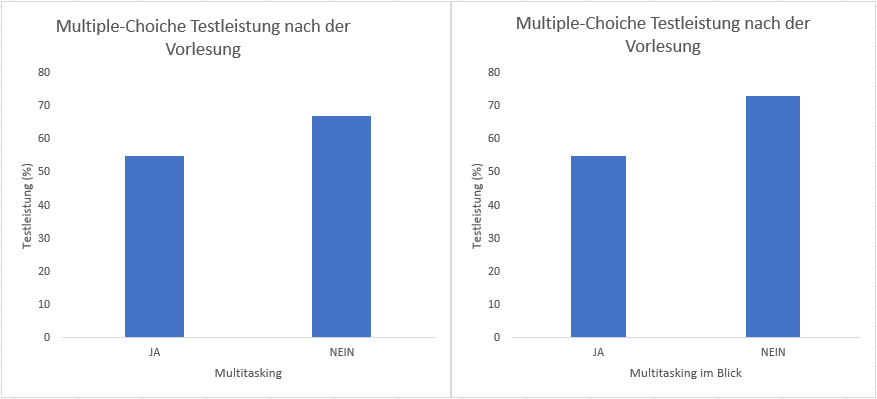
\includegraphics[scale=0.56]{images/graphtest.png}
\caption{H�ufigkeit korrekter Antworten im Test nach der Vorlesung in Abh�ngigkeit davon, ob die Studenten zugleich mit anderen Aufgaben am Computer selbst besch�ftigt waren oder nicht (linke Abbildung) bzw. davon, ob die Studenten anderen Studenten beim Multitasken am Laptop zuschauen konnten oder nicht (rechte Abbildung).}
\end{figure}


\section{Tr�bung der menschlichen Psyche}
Das Verwenden von Smartphones und Laptops st�rt das Lernen direkt durch Konzentrationsverlust w�hrend Lehrveranstaltungen und beeinflussen indirekt die akademische Leistung.

Eine Studie in Schweden von Biomedcentral Public Health \cite{Mobile} konnte  im Jahr 2011 mit 4156 Probanden aus der schwedischen Bev�lkerung, davon 1455 m�nnlich und 2701 weiblich, eine Relation erstens zwischen hohem Mobiltelefongebrauch und Stressempfinden, und zweitens zwischen Schlafst�rungen und Symptomen von Depression feststellen. Die Probanden sind in einem Alter von 20 -24 Jahren von welchen 40\% der M�nner und 48\% der Frauen studieren.  Eine weiter Studie in Schweden von Biomedcentral Psychiatrics \cite{Computer} im Jahr 2012 mit 4163 Probanden im gleichen Alter, davon 1458 m�nnlich und 2705 weiblich, untersucht die gleichen Folgen bei hohem Computergebrauch .
Beide Studien verbinden die verbrachte Menge an Zeit mit Mobiletelefone also die Konstante Erreichbarkeit oder vor dem Computer mit entweder einem Risiko f�r erh�htes Stressempfinden, Schlafst�rungen oder Entwicklung von Symptomen der Depression.
Desto mehr Zeit vor einem Bildschirm verbracht wird desto gr��er ist auch der Einfluss auf die Art wie der Mensch mit seinem Sozialen Umfeld interagiert. In Neuseeland im Rahmen einer Studie \cite{Adolescent} von PhD. Rosalina Richards, PhD Rob McGee, D.Sc Sheila M. Williams, PhD. David Welch and MD Robert J. Hancox wurden 1987\-1988, 976 Jugendliche im Alter von 15 Jahren befragt wieviel Zeit sie vor dem Fernseher verbringen und es wurde ihre Beziehung zu Gleichaltrigen und ihren Eltern bewertet mittels einer gek�rzten Version von \"Inventory of Parent and Peer Attachment\"(IPPA).
In der gleichen Studie [5] wurden 2004 3983 Sch�ller aus 144 verschiedenen Schulen die gleichen Fragen gestellt und als Erg�nzung wurden die Probanden gefragt wieviel Zeit sie vor dem Computer verbringen, wieviel Zeit sie mit Lesen und dem erledigen von Hausaufgaben in ihrer Freizeit verbringen.
In der ersten Phase 1987-1988 konnte man feststellen, dass jeder weiter Stunde vor dem Fernseher das Risiko eine schlechte Beziehung mit den Eltern zu haben um 13\% erh�ht und mit Gleichaltrigen sogar um 24\%. In der zweiten Phase 2004 war das Resultat �hnlich, mehr Zeit vor dem Bildschirm egal ob Fernseher oder Computer f�hrte zu einem h�heren Risiko eine schlechte Beziehung zu den Eltern oder Gleichaltrigen zu f�hren. Zeit mit Lesen und der Bew�ltigung von Hausaufgaben wurde hingegen mit einer besseren Beziehung zu den Eltern in Zusammenhang gebracht [5].

\chapter{Zusammenfassung und Ausblick}


%Der aktuelle Kurs  dieser weltweiten Initiativen  besteht darin, die Digitalisierung in die Schule zu integrieren. Politiker glauben, dass dies der einzige und zugleich der einfachste Weg ist  zur verbesserten Bildung.  
%Wie hier gesehen haben gibt es viele H�rden sei es auf einer gesundheitlichen Ebene, in der Grammatik oder die Implementierung von effektiven Bildungsmethoden wie die Spielifizierung des Lernens.


Durch Textverarbeitung haben sich Fehler in der Grammatik von 1980 auf 2006  bedeutend gesteigert. Die Industrie hat in dieser Instanz noch kein Optimum entsprechenden Textverarbeitungsprogramme erreicht. Laut einer Studie des Deutschen Lehrerverbands in Kooperation mit dem Schreibmotorik Institut  verlernen 80\% der Sch�ler die Handschrift, was mit regelm��igen Verwenden von Textverarbeitungssoftware korreliert. 

Konventioneller Unterricht l�sst sich auf viele Arten und Weisen anders gestalten, wie zum Beispiel auf spielerischer Ebene. Diverse Techniken erm�glichen eine Integration spielerischer Elemente in die Bildung, die Sch�ler motivieren, l�nger und effizienter zu lernen. 
Die Designprinzipien aus der Spielwelt motivieren beim Lernprozess unter anderem durch Rapides Feedback, Status und Flexibilit�t, sofern es gelingt diese zu implementieren und die passende Technologie in Klassens�len vorhanden ist. Genau diese invasive Technologie ist jedoch in  bildungsgewidmeten Infrastrukturen umstritten und bringt  Nachteile mit sich. Aus diesem Grund lenken die Rechner die Sch�ler w�hrend einer Vorlesung ab. Diese Rechner f�hren wiederum zu multitasking, was in schlechteren Testergebnissen resultiert. 

Studenten sind dauerhaft �ber digitale Ger�te wie Smartphones und Laptops  vernetzt. Dies hat einen Einfluss auf die Gesundheit und das Wohlbefinden der Gesellschaft. Vorerw�hnte Studien beweisen, dass es immer mehr abgelenkte Studenten gibt. So haben von 774 Studenten 5,6\% angegeben sich nicht anderweitig w�hrend den Lehrveranstaltungen zu besch�ftigen. Au�erdem schauen Jugendliche t�glich bis zu 150 Mal auf ihr Smartphone, das hei�t im Durchschnitt wird ihre Aufmerksamkeit alle 6 Minuten unterbrochen. Folgen davon sind: Verschlechterung der akademischen Leistung, ein erh�htes Stressempfinden und eine Isolation von der Gesellschaft.

Offenbar gibt es viele H�rden, sei es auf einer gesundheitlichen Ebene, in der Sprachlehre oder die Implementierung von effektiven Bildungsmethoden wie die Spielifizierung des Lernens. Diese H�rden k�nnen mit den richtigen Initiativen, in der Politik und zusammen mit den Lehrverb�nden �berw�ltigt werden.


Als Schlusswort schlagen wir vor, eine Weiterbildung der Lehrer zu f�rdern, die es ihnen erm�glicht, auf die H�rden der Digitalisierung aufmerksam zu machen. Die Digitalisierung in Schulklassen sollte vigilant fortschreiten um den negativen Folgen vorzubeugen. 




% ...
%--------------------------------------------------------------------------
\backmatter                        		% Anhang
%-------------------------------------------------------------------------
\bibliographystyle{geralpha}			% Literaturverzeichnis
\bibliography{literatur}     			% BibTeX-File literatur.bib
%--------------------------------------------------------------------------
\printindex 							% Index (optional)
%--------------------------------------------------------------------------
\begin{appendix}						% Anh�nge sind i.d.R. optional
   \chapter{Glossar}

\abbreviation{IPPA}		{Eine Skala die verschiedenen Qualit�ten von Jugendlichen Beziehungen mit ihren Eltern und Gleichaltrigen. Qualit�ten sind, Vertrauen, Kommunikation und Gef�hle von Groll und Entfremdung.}
			% Glossar   
\end{appendix}

\end{document}
